
%---- Created by: Sinchiguano Cesar. El Carmen - June 2022 --
\documentclass[xcolor=dvipsnames,envcountsect]{beamer}
%Default package loading
\usepackage{import}
\import{sourceFile/}{source.tex}
%--------- INTRODUCTION ----------------------
\section{Introducción}
\begin{frame}
	\frametitle{Introducción}
		\justifying
		Lorem ipsum dolor sit amet, consectetur adipiscing elit. Duis ut imperdiet lorem. Sed imperdiet sit amet quam sit amet molestie. Curabitur elementum magna sem, eu viverra augue pharetra quis. Phasellus ut turpis vel nunc fermentum ornare. Maecenas sit amet semper leo. Praesent sodales vel lectus sed hendrerit.
\end{frame}




%---------- DEFINITION/PRELIMINARY ---------------------
\section{Definiciones}
\begin{frame}
	\frametitle{Difiniciones}
\begin{definition}\label{d19} A  set $M \subseteq E(G)$ is an \emph{edge dominating set of $G$} if every $u \in E(G) \backslash M$ is adjacent to some $v \in M$. The \emph{edge domination number of $G$}, denoted by $\gamma_{e}(G)$, is the minimum cardinality of an edge dominating set of $G$. Any edge dominating set of $G$ with cardinality $\gamma_{e}(G)$ is referred to as a \emph{$\gamma_{e}$-set of $G$}.
\end{definition}
\end{frame}

\begin{frame}
		\frametitle{Definiciones}
	\begin{block}
	\justifying
		\normalfont{The sets $M_{1}=\{a, c, f\}, M_{2}=\{d, h\}$, and $M_{3}=\{a, e, g, h\}$ are edge dominating sets of $G$ in Figure 1.5. Moreover, $M_{2}=\{d, h\}$ is a minimum edge dominating set of $G$. Thus, $\gamma_{e}(G)=\left|M_{2}\right|=2$.}
		\begin{figure}[ht]
			\centering
			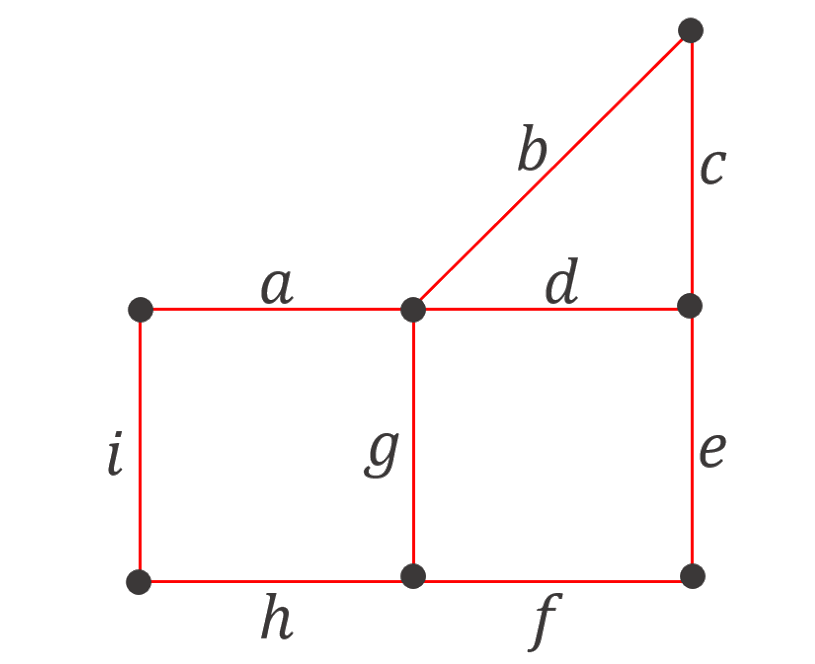
\includegraphics[width=0.35\textwidth]{./Figures/EDOM.png}
			\captionsetup{justification=centering}
			\caption{A graph $G$ with $\gamma_{e}(G)=2$.\label{edom}}
		\end{figure}
	\end{block}
\end{frame}






%----------- MAIN RESULTS ------------------------------
\section{Resultados}
\begin{frame}{Resultados}
		\begin{remark}\label{rem: 1}
		A set $S$ is an outer-connected edge dominating set of a graph $G$ if $S$ is an edge dominating set such that $H_{E(G) \backslash \mathrm{S}}$ does not have component isomorphic to $K_{2}$ or $S=E(G)$.
		\end{remark}
	\pause
	\indent To see this, consider graphs $G_{1}=P_{3}, G_{2}=P_{4}$, and $G_{3}=C_{8}$ in Figure \ref{3.1}.
	Then, $\gamma_{oce}(P_{3})=2, \gamma_{oce}(P_{4})=3$, and $\gamma_{o c e}(C_{8})=4$.
\end{frame}
\begin{frame}{Results (Cont'n)}
		\begin{figure}[ht]
		\centering
		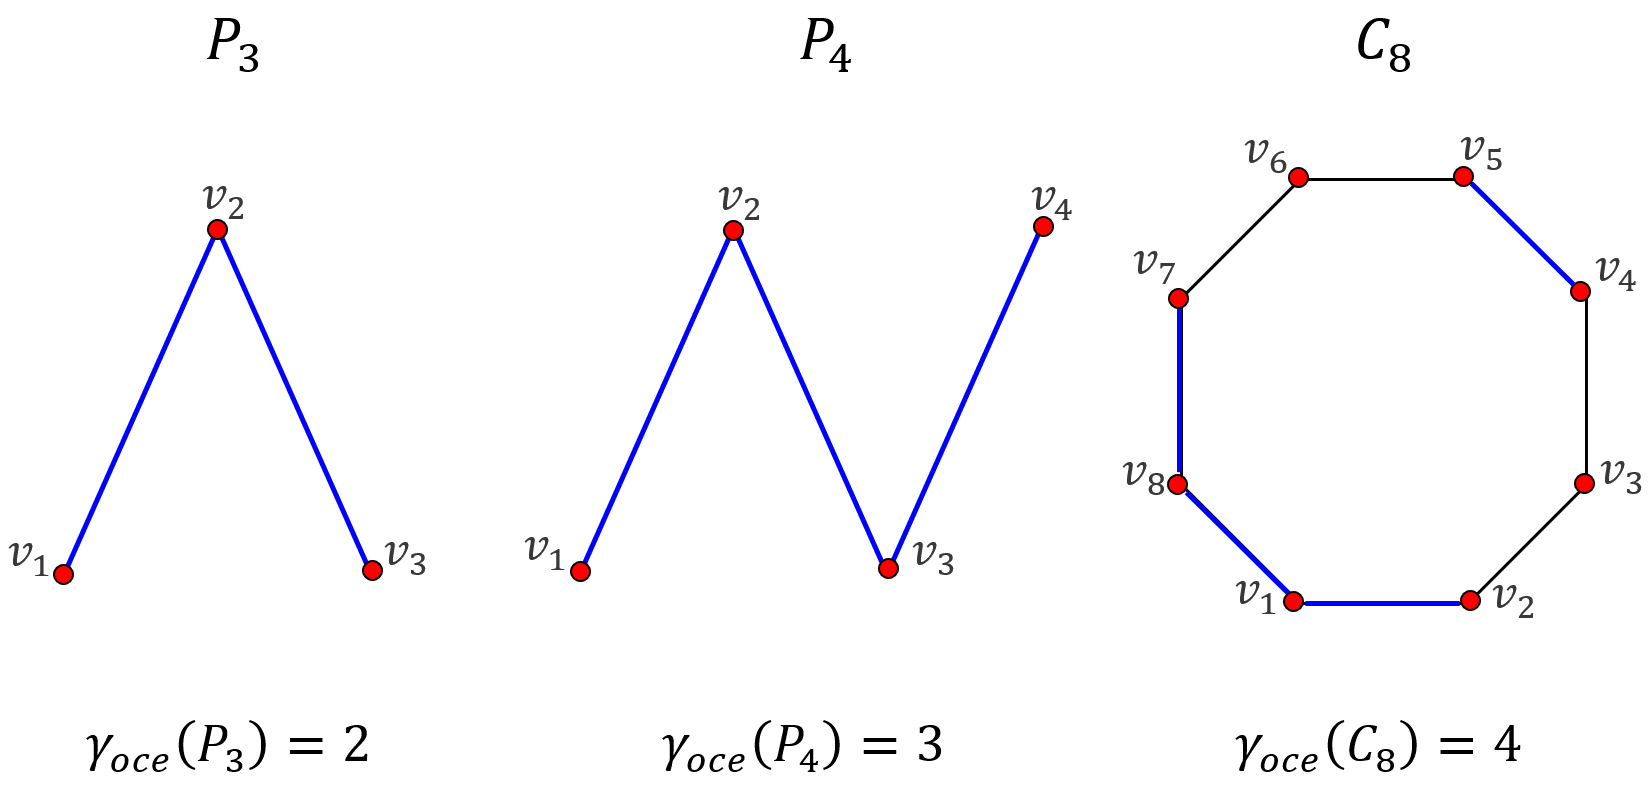
\includegraphics[width=0.9\textwidth]{./Figures/3.1.png}
		\caption{Graphs with $\gamma_{oce}(P_{3})=2, \gamma_{oce}(P_{4})=3$, and $\gamma_{oce}(C_{8})=4$.\label{3.1}}
		\end{figure} 
\end{frame}






%---------- RECOMMENDATIONS -----------------------------
\section{Recomendaciones}
\begin{frame}
	\frametitle{Recomendaciones}
	\justifying

    The following problems are suggested for further study:\\

	Lorem ipsum dolor sit amet, consectetur adipiscing elit. Duis ut imperdiet lorem. Sed imperdiet sit amet quam sit amet molestie. Curabitur elementum magna sem, eu viverra augue pharetra quis. Phasellus ut turpis vel nunc fermentum ornare. Maecenas sit amet semper leo. Praesent sodales vel lectus sed hendrerit.
\nocite{akhbari2013outer,arumugam2009connected,berge1962theory}
\end{frame}

%----------- REFERENCES  -------------
%----------- No editing in references section ----------
%----------- edit only in References.bib ----------
%	\begin{frame}[allowframebreaks]
%		\justifying
%		\frametitle{List of References}
%		\printbibliography
%	\end{frame}


%--------- THANK YOU Text --------------------------
	\begin{frame}
		\centering
		\begin{block}
			\scshape
				\begin{center}
					\Huge\emph{Gracias!}
				\end{center}
		\end{block}
	\end{frame}
%----------------------------------------------------
\end{document}
